\documentclass[twoside, 11pt, a4paper]{article}
\usepackage[latin1]{inputenc}
\usepackage[english]{babel}
\usepackage{amsmath,amsfonts,amssymb,graphicx,parskip}
\usepackage[T1]{fontenc}
%\usepackage{fourierx} % eller lmodern
\usepackage{subfigure}
\usepackage{multirow}
\usepackage{float}
\usepackage{array}
\restylefloat{figure}
\usepackage{algorithm}
\usepackage{algorithmic}
\usepackage{listings}

% for debug utskrift
\newcommand{\debug}[1]{\texttt{#1}}
% for ingen utskrift av kommentarer/debug
%\newcommand{\debug}[1]{}

\DeclareMathOperator{\erf}{erf}
\DeclareMathOperator{\erfc}{erfc}
\DeclareMathOperator{\eps}{\epsilon}
\newcommand{\dee}{\mathrm{d}}

\begin{document}
\LARGE
\begin{center}
TMA4280: Introduction to Supercomputing
\end{center}
\vspace{1in}

\begin{center}
{\bf Programming shared memory machines using \texttt{OpenMP}}
\end{center}

\Large
\vspace{0.5in}
\begin{center}
Spring 2012
\end{center}

\vspace{0.5in}

\begin{center}
\copyright Einar M. R{\o}nquist \\
Department of Mathematical Sciences\\
NTNU, N-7491 Trondheim, Norway\\
All rights reserved
\end{center}

\large

\newpage

\section{Introduction}
Thus far in the course we have considered programming parallel machines using a distributed
memory model, where several processes communicate through message passing, using
the \texttt{MPI} library. This has been the traditional programming
model used in the HPC community since distributed memory machines became popular
during the late eighties. One of the main benefits of this programming model
is that it can be used on all hardware, even machines that actually have a shared memory
architecture. However, it has one major drawback; parallelizing a code typically requires
substantial changes to the serial version.

In these notes we consider programming shared memory machines using a shared memory programming model.
In particular we consider parallelization using the \texttt{OpenMP} standard.
In later years, technology have reached a point where making a single processing core 
much faster is very challenging. In order to keep 
up with Moore's law for the next decades, vendors have started integrating several 
processing cores in one chip, even in processors targeted at desktop computers.
At the moment, dual core processors are the norm on the desktop, with quad and
hexacore processors being available in the high end market. All major vendors
have signaled that they expect 8-16 cores to be the norm within a few years, and
a few hundreds within a decade.
This means that even for desktop class programs, programmers need to start developing parallel
programs to utilize the available computing resources. The effect of this is a
substantially increased interest in developing programming tools 
which allows for code parallization on shared memory archictures with little effort.
While the \texttt{OpenMP} standard, which originated in the late ninties, initially was
aimed at HPC applications, it has now been adapted much more broadly. 
The effort to improve the standard for the desktop market has also largely benefited the 
HPC community. The increased activity has resulted in two major revisions of the standard 
in the last five years, making it quite extensive. The scope of this document is not to give 
a thorough introduction to the whole API, but rather to give an idea of the main principles,
as well as what new challenges and benefits programming using \texttt{OpenMP} offers compared to the
traditional message passing tools.
\newpage
\section{\texttt{OpenMP} programming model}
\texttt{OpenMP} is a \texttt{C}/\texttt{Fortran} language extension for programming shared memory parallel machines.
It is implemented and supported by most major vendors, including Intel, AMD, IBM and Oracle (SUN).
It is also available in open source compilers such as gcc/g++, as well as in professional versions of Microsoft Visual Studio.
Note that the clang compiler, commonly used on OSX (XCode >= 4.x) does NOT yet support OpenMP.

\begin{figure}[ht]
	\begin{center}
		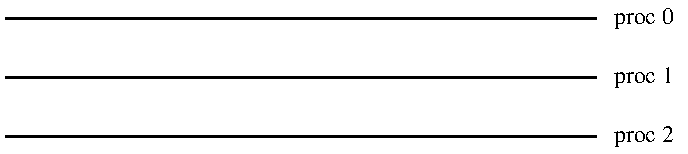
\includegraphics[width=10cm]{mpi}
	\end{center}
	\caption{An illustration of the \texttt{MPI} programming model. We have several independent
			 processes, and each of these processes have their own separate program flow.}
	\label{fig:mpi}
\end{figure}

It is built on the threading paradigm in combination with a parallel section view
of the code. This means that the main program flow happens on one processor only,
which is quite a difference from the \texttt{MPI} programming model. Consider Figure \ref{fig:mpi},
which is an illustration of the \texttt{MPI} programming model. Here we have several
processes, and each of these processes have their own separate program flow. That is, each
process is a separate instance of the program. Syncronization of these processes
is typically handled implicitly by using blocking communication calls, i.e.
if you call \emph{MPI\_Send} in one process, this process halts until
it receives a confirmation that the message has been processed. Likewise, on the receiver
end, the process blocks the program flow in the \emph{MPI\_Recv} call until it
has received the expected message.

\begin{figure}[ht]
	\begin{center}
		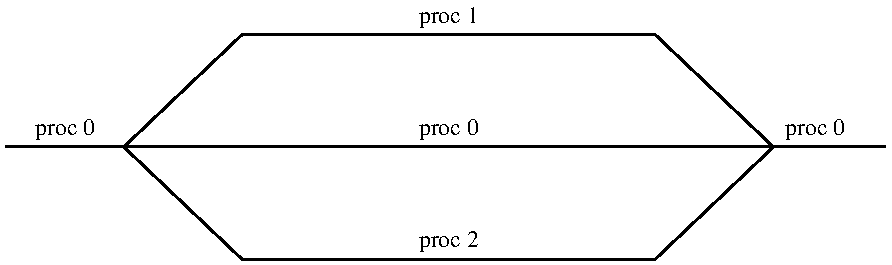
\includegraphics[width=10cm]{openmp}
	\end{center}
	\caption{An illustration of the \texttt{OpenMP} programming model. We only have a single
			 process, hence the main program flow only happens on a single processor.
			 In sections of the code that we have marked as parallel, the
			 program forks into multiple threads which work independently. At the end
			 of the parallel section, these threads join together again and the
			 program flow is returned to the first processor.}
	\label{fig:openmp}
\end{figure}
In the \texttt{OpenMP} programming model, this is different. Consider Figure \ref{fig:openmp}
which is an illustration of this programming model. \texttt{OpenMP} is based on a fork/join
programming model, where we only have a single instance of the program, i.e.
the main program flow only happens on one processor. We mark certain
sections of the program as being suitable for parallelization. When the program flow
enters these sections of the code, the program \emph{forks} into several threads which work
independently of each other. At the end of the code sections the threads \emph{join}
with the thread running on processor 0 and the program flow is returned to this single
processor. Thus in some sense one might say that the \texttt{MPI} programming model is embedded
in the \texttt{OpenMP} model, but only in those parts of the code we have marked as parallel sections. 
This is only half the truth though. In \texttt{MPI} each process have their own \emph{private} resources.
Here however, this is not true. The threads within the parallel sections all have access
to the \emph{same} resources. This is crucial to keep in mind when designating the parallel
sections of the code. One of the more common pitfalls is several threads trying to write to 
the same memory location, often due to using shared buffers during the calculations.
It is thus highly recommended that you try to design your parallel sections in such a way
that each thread has its own separate working buffers.

\subsection{Critical section}
\label{sec:critsec}

If for some reason you cannot avoid several threads needing write access to the same resources,
your only choice is to construct a critical section in your code to protect these resources.
Consider Figure \ref{fig:cs}. A critical section of the code is a section of the program in 
which only a single thread can be at any point in time. We construct such sections of the code using
a tool known as a \emph{mutual exclusion lock}, commonly referred to as a \emph{mutex}.
We make a section of the code critical by embedding it in a lock/unlock procedure.
Prior to entering the critical section of the code, the thread requests a lock of the mutex.
If the mutex is open when this is requested, the mutex is locked, and info about which thread
has the key is recorded. This mutex is now locked until the thread associated with the key
requests an unlock. The thread then moves on executing the critical section of the code.
Upon completion of the critical section the thread unlocks the mutex and continues doing 
whatever we have told it to do next.
Now, if a second thread attempts to lock the mutex while it still is locked,
the second thread will stall in the lock call until it is able to obtain the key.
Since the mutex only has a single key, it would only be able to obtain this key
after the mutex has been unlocked by the thread which is currently holding it.
Since this unlocking only happens after the critical section has been executed, we can
then guarantee that only a single thread is within the critical section of the code at any
time. We stress that this is something you should only use if there is no way around it,
since the use of a mutex leads to a \emph{serialization} of the critical section code.
This can be catastrophic for the parallel performance of your code if a large part of the
computation time is spent within such critical sections. Since this is meant to be
a brief introduction, we will not discuss these issues further in the following. 

\begin{figure}[ht]
	\begin{center}
		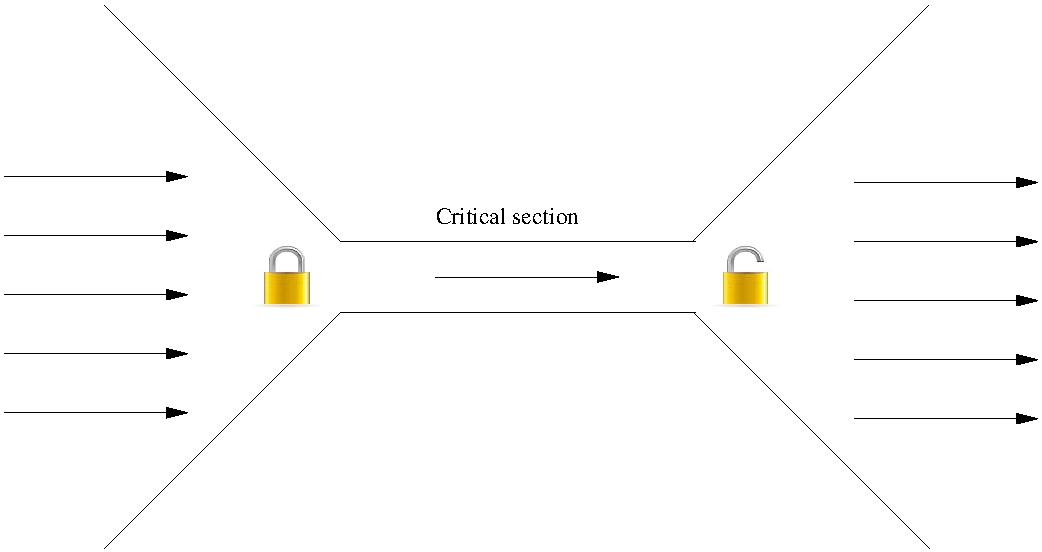
\includegraphics[width=10cm]{CriticalSection}
	\end{center}
	\caption{Illustration of a critical section. The incoming arrows represents the threads.
			 All the threads are running concurrently, until they need to enter the critical section.
			 Since only one thread can be inside the critical section 
			 at any time, the threads which want to enter need to wait until they obtain
			 the key to the mutual exclusion lock, and hence their turn to enter the code section.}
	\label{fig:cs}
\end{figure}

\section{How to use \texttt{OpenMP}}
The idea behind the \texttt{OpenMP} API is that we give the compiler instructions on which sections of the code
we want to be parallelized. This means that, in contrast to \texttt{MPI}, which works with all compilers, 
\texttt{OpenMP} requires specific support in the compiler.
The compiler then handles work division between the available number of threads. This is in stark 
contrast to \texttt{MPI} where work division is something the programmer
always have to decide up front, before modifying the serial code accordingly. 

These instructions to the compiler are known as \emph{pragma} commands. There are mainly
two classes of \texttt{OpenMP} pragmas. The first class of pragmas are those which can be used in combination 
with loop constructs such as \emph{for} loops. This is the most useful case in context 
of HPC, since the programs typically consist of multiple loops which apply the same operation
to large datasets. Consider the serial snippet
\lstinputlisting[language=C]{serial-for.c}
or, equivalently,
\lstinputlisting[language=Fortran]{serial-for.f}
in the Fortran language.

For simplicity, we here assume that DoSomething(i) does not depend on any global resources,
such as temporary working buffers. Hence this loop is highly suitable for parallelization
using \texttt{OpenMP}. In addition we first assume that DoSomething(i) has a constant cost.
To divide this loop among several threads, we simply do
\lstinputlisting[language=C]{openmp-for.c}
Here we have our first example of an \texttt{OpenMP} directive. The pragma can be broken down
into three parts
\begin{description}
	\item[\#pragma omp] - all \texttt{OpenMP} directives start with this.
	\item[parallel for] - instructs the compiler that we want the following
						  \emph{for} construct parallelized.
	\item[schedule(static)] - instructs the compiler to hand each thread approximately
							  the same number of loop iterations up front. This is a good solution
							  here since (we have assumed that) each call to DoSomething(i) has
							  the same cost. Hence such a simple division will give
							  good load balancing between the threads.
\end{description}
The ingredients in the Fortran version is the same, but the syntax is slightly different
\newpage
\lstinputlisting[language=Fortran]{openmp-for.f}
To avoid having to restate everything twice, we only give C examples in the following.

We can also run into situations where each call to DoSomething(i) has a different cost.
One example where you can run into this scenario is if DoSomething(i) consists of an
iterative method such as conjugate gradients. Each solution process can have a different
solution time. In this case, if we give each thread a fixed number of loop iterations up front,
we end up with poor load balancing between the threads. Fortunately \texttt{OpenMP}
offers a mechanism to handle these situations. We simply do
\lstinputlisting[language=C]{openmp-for-dynamic.c}
The only difference is the change of the schedule parameter in the pragma from static to dynamic. 
We here instruct the compiler to use a dynamic workload division between the threads. This means 
that we reserve one thread 
as a bookkeeper/negotiator. Within this parallel section this thread has a simple task; keep
track of which loop iterations have been performed and hand out a new one to a thread when it
requests it. Initially each thread is given a single loop iteration to perform. Once the thread
finishes this, it asks the negotiator thread for a new one. The threads keep doing this until all
work has been performed.

If DoSomething(i) is fairly costly, this works very well.
However, in some cases each DoSomething(i) may be rather cheap. In this case the cost of
asking the negotiator for a new loop iteration between every calculation may dominate the actual computation time.
\texttt{OpenMP} also offers a mechanism to try to minimize this problem. Instead of having the negotiator 
hand out a single loop iteration when a thread asks for more work, it can hand out loop iterations in chunks. 
Consider
\lstinputlisting[language=C]{openmp-for-dynamic-chunk.c}
The second parameter in the schedule (5) is the \emph{chunk size}.
This is the number of loop iterations a thread is (at most) given when it requests more work from the
negotiator thread. Thus we can limit the number of times a thread has to communicate with the negotiator,
hopefully making this part of the process less dominating.

\texttt{OpenMP} also offers a third scheduling mode, called \emph{guided}.
Consider
\lstinputlisting[language=C]{openmp-for-guided-chunk.c}

This is essentially a variant
of dynamic scheduling, where we start out with a large chunk size. The chunks are then exponentially
decreased until we reach a minimum, as specified in the chunk size. The idea here is that allocating
large chunks initially is good for performance, since these will typically overlap fairly well.
However, when the number of loop iterations left is small, we may end up in a situation where all
the remaining loop iterations are allocated to a single thread. This is bad for performance since
the other threads would then be left idle. By using progressively smaller chunks, the
chance of this happening is reduced.

The second class of \texttt{OpenMP} directives are not tied to loop constructs. Instead they are to
be used if we have sections of the code which are completely independent of each other. Consider
the snippet \lstinputlisting[language=C]{serial-sections.c}
If we are certain that these jobs are independent of each other, we can tell the compiler
this fact, and ask for the different \emph{sections} to be executed in parallel on
several threads. We do
\lstinputlisting[language=C]{openmp-sections.c}
Here each section of the code would be performed in a separate thread, before
the program flow again returns to processor 0 once all sections have been completed.
This directive is not as useful as those used in combination with loop constructs, in
particular we cannot as easily utilize a large number of threads. The reason for this
is fairly straight forward. In this example we can at most use three threads, since there
are only three sections of code specified. It is often hard to find a large number
of independent code sections to allow for a larger number of threads. Large, expensive loops,
however, are typically present in most codes.

\section{$\pi$ - \texttt{OpenMP} style}
We have previously calculated $\pi$ in both serial and \texttt{MPI} codes. We can certainly use \texttt{OpenMP}
for this as well. In the original serial code we have a loop
\lstinputlisting[language=C]{serial-integrate.c}
This is the loop where the main work happens, and is what we should focus our effort on.
In this case, it is embarassingly simple to parallelize the loop since there are no dependencies between
the loop iterations. We can simply hand a number of iterations to each thread, and then sum up the
results afterwards. \texttt{OpenMP} makes this convenient through the reduction directive
\lstinputlisting[language=C]{openmp-integrate.c}

\section{Compiling and running an \texttt{OpenMP} application}
We have a source file called \emph{openmp.c}, and we want to compile this with \texttt{OpenMP} directives enabled.
On a standard Linux computer this can be achieved by using the \texttt{-fopenmp} directive, i.e.,
\begin{verbatim}
        gcc -O3 -o openmp -fopenmp -c openmp.c
\end{verbatim}
while using the Intel compiler as we do on \texttt{Kongull/Vilje} the directive is simply \texttt{-openmp}, i.e.,
\begin{verbatim}
        icc -O3 -o poisson -openmp -c poisson.c
\end{verbatim}
As long as we do not use any \texttt{OpenMP} utility function calls,
we can still compile this code into a completely serial code, simply by removing the compiler 
switches. The compiler then simply ignore the pragmas, which makes the code look exactly as the
serial code from its point of view. This is in stark contrast to a \texttt{MPI} version
of the code where we would have to do substantial changes which makes the program dependent on the \texttt{MPI} libraries.

To run the our program using for instance 4 threads we do
\begin{verbatim}
$ OMP_NUM_THREADS=4 ./openmp 2048
\end{verbatim}

\section{Final remarks}
Modern supercomputers typically consist of multiple \texttt{SMP} nodes interconnected in a
\texttt{NUMA} organization, see the lecture notes. Clusters also fall into the same category,
since even the commodity processors used here have several cores integrated in their chips
as discussed in the introduction. In particular, \texttt{vilje} is an example of such a machine.
Here each \texttt{SMP} node consists of 16 hyper-threaded processor cores. This means that an application which
is parallelized using \texttt{OpenMP} can at most use 32 threads, although for floating point dominated
programs, running only one thread per physical core is adviced. If more computing resources
is needed, we have no choice but to resort to a distributed memory approach using 
\texttt{MPI}. The same applies to \texttt{Kongull}, except here each SMP has 12 cores, which are not hyperthreaded.

A very natural question to ask is whether or not the two approaches can
be combined. The answer to this is yes. In fact this approach often allows us the best of
both worlds. Fine-grain parallelism is often intricate to exploit using a distributed memory 
model, while the convenience offered by the shared memory model often makes it fairly trivial
to express. In addition, it is not always easy to say up front where exploiting fine-grained
parallelism actually will improve the performance of your program.  Since the modifications
to the program using the \texttt{OpenMP} approach is minimal, we do not have to
invest much effort just to benchmark whether or not parallizing a particular loop improves
performance.

Coarse-grain parallelism, however, is often fairly involved to exploit using a shared
memory model, in particular due to the complications involved in protecting shared resources
such as working buffers. This often lead to excessive memory usage or serialization of
substantial parts of the code through usage of critical sections, see Section \ref{sec:critsec}.
Using a distributed memory model, this problem is nonexistent. Each process have 
their own private resources which are inaccessible from the other processes.
Here expressing coarse grain parallelism is often just a matter of adjusting the limits
on some loops, as well as adding the appropriate library calls for data exchanges
between the processes when such exchanges are needed.

Hence a program where we utilize a message passing based approach, i.e. \texttt{MPI}, to
express the coarse grain parallelism, while utilizing \texttt{OpenMP} pragmas to express
the fine grain parallelism within each \texttt{MPI} process allows use to use each
approach for what they are best at, while avoiding their weak sides.
\newpage
\section{Further reading}
You can find the official \texttt{OpenMP} homepage at \emph{http://www.openmp.org}. This page is a great
resource for those who are interested in more details. In addition to having the description
of the standard, it also contains links to several books on subject, as well as discussion forums
where you can ask questions. If a source of tutorials are to be suggested,
we can recommend \emph{https://computing.llnl.gov/tutorials/openMP/}.

\bf Acknowledgement\rm. Stephan Diederich helped with proof reading
and gave some valuable input while this introduction was written.
This document is written by Arne Morten Kvarving. Your assistance was greatly appreciated.
\nocite{openmp}
\nocite{openmptut}
\bibliographystyle{plain}
\bibliography{referanser}
\appendix
\section{\texttt{OpenMP} implementation of a program calculating $\pi$ using an integral.}
\label{app:openmp-integrate}
\lstinputlisting[language=C,basicstyle=\small]{serial.c}
\end{document}
